Time Response is sum of two responses: the natural response and the forced (kamel) response. \textit{natural response} is response of system to dirac delta on the other hand, \textit{forced response} is the response of system from applying an external force. To understand it in qualitatively manner remember what you know about a differential equation.
%\nicefrac{at}{2}
\subsection{Formulas}
\begin{minipage}{0.4\linewidth}
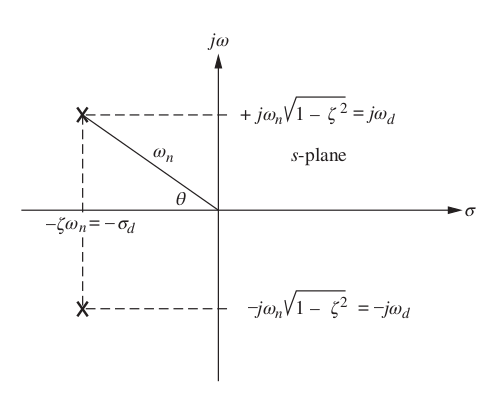
\includegraphics[width=0.8\columnwidth]{Resources/keesy.png}
\captionsetup{width=0.8\textwidth}
\centering
\end{minipage}
\begin{minipage}{0.6\linewidth}
$$ C(s) = \frac{\omega_n^2}{s^2+2 \sigma s + \omega_n^2} ~~ , ~~ c(t) = 1 - e^{ - \sigma t} \Big (cos(\omega_d t) + \frac{\sigma}{\omega_d} sin(\omega_d t) \Big)$$ 
$$ \zeta = \frac{\sigma}{\omega_n} ~~ , ~~ cos \theta = \zeta $$
$$ T_P = \frac{\pi}{\omega_d} ~~ , ~~ T_s = \frac{4}{\sigma}$$~
%$$ \%OS = \frac{c_{max}-c_{final}}{c_{final}} \times 100 ~~ , ~~ \%OS = \big  {e^{\mathlarger {-\sigma T_P}}} \times 100 $$
$$ \%OS = \frac{c_{max}-c_{final}}{c_{final}} \times 100 ~~ , ~~ \%OS = \big  e^{-\sigma T_P} \times 100 $$
\end{minipage}
~\\
%\scalebox{1.5}{\sfrac{3}{2}}


\subsection{Steady-Space Error}
For unity feedback systems, $e(\infty)$ Steady-Space Error defined as
$$ e(\infty) = \frac{1}{1+K_p} ~~ , ~~ e(\infty) = \frac{1}{K_v} $$
$$ e(\infty) = \frac{1}{K_a} $$~\\
where \\
$$ K_p = \lim_{s \to 0} G(s) ~~ , ~~ K_v = \lim_{s \to 0} s G(s) ~~ , ~~ K_a = \lim_{s \to 0} s^2G(s)$$~\\
and $G(s)$ is forward open loop transfer function

Hi somik
Thanks for your reply
Somik you are indeed right, I added MX Record as you said and after looking into my google apps there is an option for handling non-SSL too.

I Just wanted to verify this fully so it take me time and I decide to post answer after that.
Nevertheless, the slow response of server is mysterious.
So as Genesis suggested, waiting for technical admin is the best

Again thanks for your kind help.

Regards,
Bijan
